\documentclass[oneside]{article}


\usepackage{textcomp}
%change font. (ALTERNATIVE:  mathpazo, mathptmx, helvet, avant, courier, chancery, bookman, newcent, charter)
\usepackage{charter} % math & rm 
\normalfont
\renewcommand{\ttdefault}{lmtt} %tt

\usepackage[utf8]{inputenc}
\usepackage[italian]{babel}
\usepackage[T1]{fontenc} % Use 8-bit encoding that has 256 glyphs
%\usepackage[latin3]{inputenc}
%\linespread{1.05} % Line spacing - Palatino needs more space between lines
\usepackage{microtype} % Slightly tweak font spacing for aesthetics
\usepackage[hmarginratio=1:1,top=32mm,columnsep=20pt]{geometry} % Document margins
\usepackage{multicol} % Used for the two-column layout of the document
\usepackage[hang, small,labelfont=bf,up,textfont=it,up]{caption} % Custom captions under/above floats in tables or figures
\usepackage{booktabs} % Horizontal rules in tables
\usepackage{float} % Required for tables and figures in the multi-column environment - they need to be placed in specific locations with the [H] (e.g. \begin{table}[H])
\usepackage{hyperref} % For hyperlinks in the PDF
\usepackage{lettrine} % The lettrine is the first enlarged letter at the beginning of the text
\usepackage{paralist} % Used for the compactitem environment which makes bullet points with less space between them
\usepackage{lipsum} % Package to generate dummy text throughout this template
\usepackage{graphicx}
\usepackage{enumitem}   

%abstract
\usepackage{abstract} % Allows abstract customization
\renewcommand{\abstractnamefont}{\normalfont\bfseries} 
\renewcommand{\abstracttextfont}{\normalfont\small} 

%titolo
\usepackage{titlesec} 
\renewcommand\thesection{\Roman{section}}
\renewcommand\thesubsection{\Roman{subsection}} 
\titleformat{\section}[block]{\Large\bfseries\scshape\centering}{\thesection.}{1em}{} 
\titleformat{\subsection}[block]{\large\scshape}{\thesubsection.}{1em}{} 
\titleformat{\subsubsection}[block]{\scshape}{\thesubsubsection.}{1em}{} 




%headers & footers 
\usepackage{fancyhdr} % Headers and footers
\pagestyle{fancy} % All pages have headers and footers
\fancyhead[L]{\bfseries{{\textsf{Davide Tedesco}}}}
\fancyhead[R]{\bfseries{{\textsf{$\bullet$ Verso una nuova frontiera della
 chitarra classica $\bullet$ }}}}
%\fancyhead[R]{\small \leftmark}
\cfoot{\thepage}




%----------------------------------------------------------------------------------------
%	TITLE SECTION
%----------------------------------------------------------------------------------------
\thispagestyle{empty}


\title{\vspace{-15mm}\fontsize{24pt}{10pt}\selectfont\textsf{\bfseries{\textsc{Verso una nuova frontiera della
 chitarra classica}}}} % Article title

\author{
\large
\textsc{Davide Tedesco}\\
\small{SMERM - Conservatorio di Musica di Roma, Santa Cecilia}\\
\small \href{mailto:me@davidetedesco.it}{\texttt{me[at]davidetedesco[dot]it}} 
%\vspace{-5mm}
}


\date{Luglio 2020}

%----------------------------------------------------------------------------------------




\begin{document}

\maketitle % Insert title

\tableofcontents

\thispagestyle{empty} 

%----------------------------------------------------------------------------------------
%	ABSTRACT
%----------------------------------------------------------------------------------------

\begin{abstract}

Le possibilità donate dall'arte musicale elettronica combinate con quelle tradizionali hanno portato la composizione per strumento solo a crescere per importanza e creatività, sia per l'interesse mostrato dai compositori, che per la dedizione degli esecutori allo sviluppo di un nuovo linguaggio oltre quello proprio del repertorio tradizionale. Questo atteggiamento è particolarmente visibile nell'ambiente chitarristico, nel quale non solo compositori di professione, ma anche gli strumentisti hanno iniziato a porre la questione del \textit{come} possa essere interpretata la loro performance all'interno di un discorso musicale contemporaneo. La chitarra, che di sua natura si presta a vari utilizzi, viene dunque paragonata spesso a soli gesti virtuosistici che non nutrono un vero senso compositivo ma solamente \textit{muscolare} alimentando un discorso compositivo che porta la qualità dei manufatti musicali sempre più verso la semplicità e immediatezza di esecuzione. Il compositore contemporaneo osservando l'ambiente che lo circonda, annotandosi i punti di forza della musica attuale ed estendendo le possibilità pratiche che un esecutore gli propone deve quindi cercare di implementare il suo \textit{modus operandi} alla scrittura non limitandosi ai confini imposti dall'esecutore. Il seguente testo mira dunque ad avviare una ricerca scientifico-compositiva volta a donare nuovo splendore alla chitarra classica, mostrando ed ampliando le capacità espressive dell'esecutore estendendole attraverso l'utilizzo di adeguati mezzi elettronici.

\end{abstract}



%----------------------------------------------------------------------------------------
%	ARTICLE CONTENTS
%----------------------------------------------------------------------------------------
\newpage
\begin{multicols*}{2} % Two-column layout throughout the main article text



%-----------------------------------------------------1= Introduzione
\section{ Introduzione}
\noindent

La chitarra è forse lo strumento che nelle varie epoche più si è adattato e piegato al volere e alla necessità di chi lo adoperava; è stato allo stesso tempo un mezzo diffuso nell'ambito popolare ed in quello colto subendo cambiamenti costruttivi sostanziali ma mantenendo sempre la massima praticità. Se in ambito colto venne molto apprezzato nel 1600, 1800 e dalla metà del 1900, in ambito popolare è divenuto forse lo strumento musicale per eccellenza ed è stato oggetto di un boom di vendite  e di apprezzamento tuttora in atto. Grazie alla sua mutevole e sempre interessante predisposizione all’incoronazione di miti pop per mezzo della sua versione elettrica ha fatto da padrone nelle vite musicali di molti giovani e non giovani. Lo strumento originario oltre le sue possibilità di esecuzione per mezzo di eccitazione delle corde è stato negli anni studiato e re-interpretato e ne sono conseguiti sviluppi multipli. Da un lato l’ambito percussivo è stato esplorato con brani quali \textit{Ko-Tha} di Scelsi e dall’altro l’amplificazione dello strumento acustico ha reso possibile l’emersione di timbriche e sonorità non percepibili(ascolto del \textit{microcosmo} timbrico), facendo sviluppare notevolmente il fenomeno del \textit{tapping}\footnote{Visionato dal pubblico italiano per la prima volta in uno storico video che ritrae Vittorio Camardese, medico di professione, ma esperto di tapping per hobby, \href{https://www.youtube.com/watch?v=UmTQYquqxSY}{visible a questo link}} e della ricerca sulla sola tastiera. Numerosi sono inoltre gli utilizzi e le possibilità donate dall’elettrificazione e dal radicale re-styling che portati all’interno della musica colta come mezzi post-avanguardistici hanno dato luogo quasi ad una \textit{corrente della chitarra elettrica contemporanea} con autori quali Romitelli\footnote{Trash TV Trance, 2002} e Murail\footnote{Vampyr!, 1984}. 
La domande che sorgono dunque da questa prima panoramica sono le seguenti: qual è il ruolo della chitarra (classica, elettrica e in tutte le sue versioni) nella musica contemporanea oggi? È ancora uno strumento attuale? Quale deve essere l’atteggiamento del compositore verso uno strumento usato tanto per il suo repertorio popolare, quanto per il suo repertorio classico?

%----------------------------------------------------2= La chitarra

\section{ Breve storia della chitarra}
\hspace*{10mm}

Dalla famiglia dei liuti nel 500 d.C. circa, si iniziarono a intravedere alcune delle più moderne versioni dello strumento con il guscio\footnote{ovvero la cassa armonica} non più di forma tondeggiante, esso fu sostituito successivamente da due superfici piatte unite da una fascia lungo i bordi.

\includegraphics[width=0.4\textwidth]{img/chit_spaccato.png}

\noindent
Anche se l’origine della chitarra ci indica che essa provenga dal liuto, con il passare dei secoli lo strumento ha cambiato varie volte nome e già nel XIV secolo veniva descritto con il nome di \textit{chitarra moresca} in un antico libro spagnolo\footnote{Curt Sachs, Storia degli strumenti musicali, Mondadori 1980}. In seguito venne denominata \textit{mandola}.
Questa famiglia strumenti a corda pizzicata, veniva suonata attraverso un plettro od una penna, e gli strumenti facenti parte della stessa avevano spesso quattro corde a simboleggiare le quattro fasi della luna, le settimane del mese o un qualche significato spirituale particolare. Gli accordi, o in ogni caso il modo di suonare simultaneamente più corde era in quel periodo sconosciuto ai più, e lo strumento era suonato inizialmente solamente per eseguire una melodia e solo occasionalmente vi venivano eseguiti degli ostinati per accompagnare la melodia. Con il passare dei secoli e dei luoghi in cui lo strumento fu utilizzato e sviluppato, le sapienze orientali e occidentali si mescolarono fino divenire in Andalusia il liuto che conosciamo\footnote{Ibidem}.
Il liuto divenne quindi lo strumento predominante in Europa tra 1500 e 1700,  ed anche se in quel periodo in Spagna non era molto apprezzato dall’aristocrazia, la musica popolare spagnola lo fece conoscere al resto d’Europa. La musica colta, al contrario, veniva eseguita su di una \textit{vihuela}\footnote{antico strumento musicale della famiglia dei liuti} la più usata era in genere la \textit{vihuela da mano} che si differenziava dalla \textit{vihuela da arco}\footnote{essa veniva suonata appunto con un arco} per il modo in cui la si suonava; la vihuela da mano aveva in genere 6 o 7 corde ed era accordata in vari modi\footnote{Ibidem}.\newline
L’arte liutistica ebbe il suo declino verso la fine del ‘600 quando gli strumenti a tastiera iniziarono a prendere piede, ma con l'eclissarsi del liuto la chitarra iniziò ad essere più apprezzata, soprattutto per la sua maneggevolezza e facilità di trasporto.
Sui principi del '600 la chitarra aveva solamente quattro corde doppie, che spesso venivano accordate in “Do-Fa-La-Re” o “Fa-Si-Re-Sol”. 
In questo periodo la chitarra aveva la cassa armonica più stretta e profonda e non come la conosciamo oggi.
La chitarra italo-spagnola incominciò a viaggiare in Europa arrivando prima di tutto all’aristocrazia francese, dove venne molto apprezzata.
La chitarra divenne dunque uno strumento per dilettanti e la sua struttura fu semplificata, sei corde singole e non più doppie con l'accordatura “Mi-La-Re-Sol-Si-Mi” che ancora oggi utilizziamo.
Nell’800 venne poi introdotta un'ulteriore miglioria con la sostituzione dei piroli in legno con quelli a viti in metallo.\newline
La chitarra ebbe dunque alti e bassi nella sua diffusione e nel gradimento che seppe riscuotere, fu riportata a dei livelli altissimi, in ambito colto, grazie all’apporto di figure quali Andrés Segovia, Joaquin Rodrigo e Heitor Villa-Lobos.


%----------------------------------------------------3= La chitarra nella musica contemporanea

\section{ La chitarra nella musica contemporanea}
\noindent

Iniziando a scavare all'interno della storia della composizione per questo strumento, non si può far altro che passare per i classici oramai intramontabili che ogni studente di Conservatorio incontra e studia assiduamente oltre ai tre grandi nomi già citati, ci si ritrova ad osservare scaffali interi dei negozi in cui sono inseriti centinaia di studi per chitarra di autori classici quali: Sor, Giuliani, Carulli e via dicendo. Non dobbiamo dunque stupirci del fatto che in sede di concerto il chitarrista tenda a realizzare una \textit{gara all'esecuzione più veloce}, poichè la premessa didattica è sempre stata improntata alla ricerca della velocità di esecuzione e al virtuosismo. Ciononostante, è 
possibile individuare esecutori in grado di interpretare e contestualizzare un'opera che, se pur rari, rappresentano autentiche gemme nel contesto del panorama musicale, in quanto capaci di colmare di forma e sostanza le composizioni per chitarra sola. Ne sono esempi Arturo Tallini\footnote{Napoli, 1958},  Elena Casoli\footnote{Milano, 1962} e Ruben Mattia Santorsa\footnote{Potenza,1992}, oltre a molti altri esecutori eccezionali nel panorama internazionale, che attraverso la collaborazione proficua con compositori, alunni e conservatori riescono a delineare progetti dal più largo respiro donando uno spazio congruo per la chitarra all'interno della \textit{giungla} musicale odierna.
%\begin{figure}
\includegraphics[width=0.5\textwidth]{img/ektopos.png}
%\caption{Agostino Di Scipio - Ektopos}
%\label{img/ektopos.png}}
%\end{figure}
L'ambiente chitarristico rivela dunque alcuni dei suoi gioielli proprio attraverso esecutori che sono riusciti a comprendere il ruolo che il proprio strumento può avere e ponendosi con occhio e orecchio vigile allo studio delle partiture contemporanee. Se da un lato ci si aspetterebbe un vasto repertorio chitarristico contemporaneo ricco di idee e nuove possibilità, da un certo punto di vista si rimane delusi, trovando opere realizzate da grandi e rinomati compositori quali Berio\footnote{Sequenza XI}, Ferneyhough\footnote{No time} e Maderna\footnote{Y Después}, che rispecchiano però un'idea di composizione per strumento solo \textit{primo-novecentesca}. Si trovano invece spunti di riflessione brillanti in compositori a noi più vicini come Di Scipio\footnote{Ektopos, in figura}, Murail\footnote{Tellur} e Romitelli\footnote{Solare, Seascape ed altre opere}. Sebbene le composizioni di questi autori riescano in qualche modo a dar giustizia alle sei corde, troviamo nel brano di Scelsi \textit{Ko-Tha}\footnote{del 1962} una più vasta ricerca sul suono e una prima esperienza chitarristica percussiva che cerca di sfruttare lo strumento in maniera non convenzionale. Dall'ascolto delle registrazioni \textit{scelsiane} custodite nell'archivo della \textit{Fondazione Isabella Scelsi} notiamo dunque una vera e propria ricerca del e sul suono che si avvicina al \textit{microcosmo timbrico} più di quanto altri compositori dopo di lui siano riusciti a realizzare. Dunque l'utilizzo dello strumento come una percussione, degli strappati e delle possibilità al di fuori del melodico iniziano veramente a ristrutturare la concezione compositiva dello strumento. %La ricerca e la risposta di Berio è invece (come in tutte le sue sequenze) una \textit{creazione di un virtuosismo} che punta al far esperire la chitarra e le sue capacità melodico-armoniche al massimo delle sue possibilità. 
Questo utilizzo della chitarra classica all'interno dell'ambito contemporaneo riesce a tagliare la tela della tradizione, e le esperienze menzionate in precedenza di interventi musicali con la chitarra elettrica\footnote{Trash TV Trance e Vampyr!}, entrano possentemente all'interno del paesaggio musicale, rendendo ben visibili le possibilità timbriche, compositive e teatrali che uno strumento popolare quanto diffuso può raggiungere. Non è un caso che le composizioni per chitarra elettrica di Murail e Romitelli siano costantemente suonate, proposte e pubblicate sul web ed in programmi di sala. 
Se dunque questo strumento \textit{rivisitato} è riuscito a portare tanta novità, apprezzamento e polemica, perché la chitarra classica rimane sempre più nell'ombra in ambito contemporaneo?
L'utilizzo dell'elettronica all'interno del panorama musicale per strumento solo è come se fosse vista quindi come un di più, da poter incollare o porre come sfondo al suono dello strumento, rendendo di fatto una manciata le composizioni per chitarra classica ed elettronica sensate realmente efficaci.

%----------------------------------------------------4= L’aumentazione: l'amplificazione, Il feedback e la distorsione

\section{ L’aumentazione}
\noindent

In questo vasto ambiante compositivo ed esecutivo che porta con sé brillantezza e freschezza di idee, vi è però sempre un minimo comun denominatore, ovvero lo strumento solo lasciato alle sue possibilità fisiche che ha reso oramai stereotipato il modo di scrivere per lo stesso. Forse si può notare nella mancanza dell'elettronica all'interno del discorso compositivo chitarristico classico, una voglia di legame con il passato che sta portando a lungo andare alla dispersione dei risultati raggiunti nel '900, lasciando lo strumento in mano alla sola musica popolare.\newline

\noindent Da queste riflessioni nasce dunque la necessità di provare a realizzare una musica che possa integrare l'elettronica con lo strumento, come è già stato fatto per molti altri strumenti, riuscendo a captare il microscopico dello strumento, le sue caratterizzazioni fisiche e le possibilità donate dall'esperienza della chitarra elettrica nel contemporaneo. Il processo che nasce da questi pensieri può esser inteso come una vera e propria \textit{aumentazione} dello strumento che attraverso l'elettronica e la gestione del gesto musicale per mezzo dell'elettronica riesce a donare nuove possibilità allo stesso. La ricerca in atto porta dunque alle prime tre possibilità che il sistema sperimentato mette a disposizione: 
\begin{enumerate}[label=(\roman*)]
\item L'amplificazione
\item Il feeback 
\item La distorsione
\end{enumerate}

\subsection{L'amplificazione} 
Il posizionamento di un sensore piezo-elettrico sul \textit{piano armonico} dello strumento è un'operazione non nuova nell'ambito chitarristico. Laddove esso viene utilizzato come mero sistema per \textit{realizzare uno zoom sullo strumento} in situazioni in cui esso risulterebbe flebile ed impercettibile, esso viene utilizzato solamente come mezzo di amplificazione puro(senza un'intermediazione coscente) che ad un livello di amplificazione costante porta il suono nel modo più chiaro possibile agli ascoltatori. Tuttavia, una simile soluzione tecnica non porta con sé l’esperienza di Stockhausen in \textit{Mikrofonie I}\footnote{usando il microfono come strumento} che viene così relegata 
al dimenticatoio. Infatti, l'utilizzo di un microfono a contatto e la gestione dello stesso in tempo reale è forse il modo più immediato, chiaro e apprezzabile di operazione ed emulazione dell'osservazione al microscopico.

\includegraphics[width=0.4\textwidth]{img/chit.jpg}

Le unghie, i polpastrelli ed il palmo della mano sono eccitatori talmente vari che è possibile apprezzarne chiaramente la differenza solamente attraverso l'amplificazione, rendendo chiaro ciò che già da un paio di metri di distanza in ambito chitarristico non è più percepibile. La gestione attraverso il filtraggio del suono in tempo reale rende ancor meglio l'idea di cosa due strumenti(la chitarra ed il microfono) possano realizzare, donando nuove sonorità e timbriche allo strumento chitarra, e dando la possibilità di maggior dinamicità, senza appiattirsi alla importante ma pur limitata esperienza polpastrello-unghia descritta da Pujol\footnote{Emilio Pujol, El dilemmma del sonido en la guitarra, Ricordi 1979}.

\subsection{Il feedback} 
Da anni utilizzata come tecnica di aumentazione nell'ambito della chitarra elettrica, seppur classificabile in diverse tipologie è forse una delle frontiere da esplorare nell'ambiente musicale chitarristico classico. Il feedback di natura diversa\footnote{feedback digitale; feedback di natura acustica; feedback di natura strutturale}, può essere implementato strutturalmente sullo strumento per mezzo di 2 componenti: \begin{enumerate}\item un sensore piezo-elettrico\item un attuatore\footnote{altoparlante senza membrana in grado di propagare strutturalmente il suono} \end{enumerate} Essi realizzano un vero e proprio sistema di feedback strutturale gestibile dall'esecutore e limitato solamente dalla natura fisica dello strumento che viene utilizzato. Attraverso una IR\footnote{risposta all’impulso, ovvero fotografia di come reagisce un corpo risonante ad un impulso} riusciamo dunque a determinare le zone frequenziali in cui il sistema risponde meglio alle sollecitazioni effettuate da particolari frequenze che emergono attraverso questa retroazione strutturale.
\newline

\includegraphics[width=0.4\textwidth]{img/ir.png}
\noindent
Nell'immagine esemplificativa notiamo la curva della risposta in frequenza del sistema in quella che chiameremo \textit{posizione 1}(nel seguito della ricerca verranno adoperate varie posizioni per esplorare e definire la differenza tra le varie posizioni del sistema), ovvero l'accoppiamento di sensore e attuatore in due precisi luoghi. Come è possibile visionare nel video esemplificativo\footnote{\href{https://www.youtube.com/watch?v=7BwwTopM3Ek}{Link al video d'esempio della gestione del feedback}}, la gestione del feedback sullo strumento risulta adeguata a seconda dei movimenti dell'esecutore, i quali catalogati e studiati rientreranno all'interno dei gesti da implementare in partitura(ed esplicati in legenda), facendo raggiungere una nuova consapevolezza dello strumento al musicista. I primi limiti che si pongono con il feedback sono però le frequenze a cui lo strumento riesce a risuonare(dipendenti dallo strumento, dalla sua grandezza, forma, materiali, costruzione e dal sensore ed attuatore utilizzati), i quali vengono però aggirati attraverso l'implementazione di filtri che rendono più malleabile l'utilizzo del feedback stesso. La tipologia di filtro utilizzato va ovviamente a far emergere caratteristiche diverse nella realizzazione sonora-timbrica, ma non potrà mai far realizzare un qualcosa di totalmente estraneo alla fisicità dello strumento in uso, e ciò renderà sicuramente ogni esecuzione unica, ma denotando un unico luogo di provenienza acustica e compositiva, facendo quasi divenire la chitarra un\textit{compressore delle azioni dell'interprete} dal lato del feedback.

\subsection{La distorsione} 
Dopo aver realizzato che la chitarra può essere aumentata riuscendo a far espletare nuove sonorità, timbri e metodologie di esecuzione si è pronti al passo successivo, ovvero cercare di far appropriare lo strumento originario, delle tecniche e delle possibilità della chitarra elettrica. Nell'esempio in video\footnote{\href{https://www.youtube.com/watch?v=K3yqyxcJStg}{Link al video d'esempio della distorsione}} si nota come l'implementazione e la gestione della distorsione sia non solo possibile e funzioni molto bene, ma come essa riesca a portare con naturalezza un elemento come quello della distorsione nel contesto chitarristico. La chitarra di per sé è infatti ora equipaggiata delle possibilità che la chitarra elettrica detiene (attraverso il sensore piezo-elettrico), e la distorsione come mezzo espressivo riesce a fondere la tecnica e i timbri sviluppati nell'ambito popolare degli ultimi 100 anni con le consuetudini e le corde in nylon della chitarra classica. Questo ultimo passaggio all'interno del discorso di \textit{aumentazione} dello strumento rinnova notevolmente le possibilità ed insieme al feedback ed alla \textit{microfonazione compositiva} dona nuova linfa ad uno strumento troppo spesso sottovalutato.


%\vfill\null
%\columnbreak
%----------------------------------------------------5= Gli Sketches e gli Studi per chitarra
\section{ Gli \textit{Sketches} e gli \textit{Studi} per chitarra}
\noindent

Alla ricerca non di un nuovo strumento, bensí di una nuova tipologia di scrittura e ricerca di un nuovo virtuosismo, non basato sulla sola velocità dell’esecuzione dei brani, e  sfruttando l'\textit{aumentazione} appena descritta si giunge allo sviluppo dei primi esempi compositivi.
Il primo approccio in questo percorso è consistito nella realizzazione di \textit{Sketches}\footnote{\href{https://github.com/SMERM/BN-Tedesco/blob/master/COME-02/Lezioni_in_Compresenza/20200324/Sketches.pdf}{Link agli Sketches}}, ovvero appunti con delle prime idee che potevano essere realizzate sullo strumento prima dell'implementazione del sistema elettroacustico. Con esse sono sorte alcune questioni puramente di scrittura sul \textit{come} rappresentare chiaramente i movimenti delle due mani, i \textit{luoghi percussivi} sulla chitarra ed il rapporto e la scrittura dell'elettronica.
La scrittura per mezzo di due pentagrammi ha reso perfettamente il senso di contemporaneità dei gesti fra le mani, fungendo per la mano sinistra da pentagramma tradizionale, mentre per la mano destra da un'intavolatura\footnote{essa veniva utilizzata nel passato come metodologia di scrittura liutistica, ed oggi è usata per imparare a suonare} non per le corde ma per le dita. 

\includegraphics[width=0.4\textwidth]{img/legenda.png}
\noindent
L'intavolatura per la mano destra riporta sul pentagramma i luoghi numerati che fanno riferimento al piano armonico(in figura) che possono esser combinati con le dita o le parti della mano destra. In questa intavolatora i cinque righi vengono utilizzati per le cinque dita della mano. 

\includegraphics[width=0.4\textwidth]{img/luoghi_perc.png}
\noindent
I \textit{luoghi percussivi} numerati sono molto diversi dal punto di vista della resa percussiva ed hanno spettri frequenziali variegati, essi possono essere cosí brevemente descritti:
\begin{enumerate}
\item $\longrightarrow$Profondo e risonante 
\item $\longrightarrow$Rotondo e risonante
\item $\longrightarrow$Secco e medio-alto
\item $\longrightarrow$Chiaro e deciso
\end{enumerate}

L'esperienza degli \textit{Sketches} ha fatto nascere delle prime risposte compositive all'interno degli \textit{Studi} per chitarra sola, che riportano a livello pratico alcune delle esperienze avute durante l'importante periodo iniziale di ricerca. Essi ad oggi sono quattro e riportano 4 tipologie di timbrica e realizzazione diversa.
L'importanza della scrittura di studi, che nella storia della musica sono interpretati a livello compositivo molto vario(dagli studi prettamente tecnici a quelli totalmente compositivi e intrisi di sperimentazione della scrittura), fa sì che l'interprete divenga sempre più consapevole, a piccoli passi, della totalità di prospettive sonore disponibili e velate nel suo strumento. All'interno di questo progetto di molto ampio respiro, il \textit{primo studio}\footnote{\href{https://github.com/SMERM/BN-Tedesco/blob/master/COME-02/Lezioni_in_Compresenza/20200331/Draft_1_Studio_n.1_Audio.wav}{Link all'audio}} non fa uso dell'elettronica bensì della voce dell'interprete(oltre allo strumento), lasciando trasparire una volontà di ricerca all'interno dell'interprete insieme a quella all'interno dello strumento. Nel \textit{secondo studio}\footnote{\href{https://github.com/SMERM/BN-Tedesco/blob/master/COME-02/Lezioni_in_Compresenza/20200407/Draft_1\%20Studio\%20n.2\%20Partitura.pdf}{Link alla partitura}} l'amplificazione viene utilizzata per la prima volta in combinazione con il sensore e l'attuatore che oltre che per l'amplificazione viene utilizzato come un emettitore di suoni pre-registrati. È però nel \textit{terzo}\footnote{\href{https://github.com/SMERM/BN-Tedesco/blob/master/COME-02/Lezioni_in_Compresenza/20200519/Appunti_Studio_n.3_a.jpeg}{Link agli appunti del terzo studio}} e \textit{quarto studio}\footnote{\href{https://github.com/SMERM/BN-Tedesco/blob/master/COME-02/Lezioni_in_Compresenza/20200616/Studio_n.4_a.pdf}{Link alla partitura}} che il feedback inizia a presentarsi nella sua potenza espressiva. La distorsione del terzo studio ed il Feedback oltre che la scordatura denotano degli elementi in più che l'interprete deve studiare così da capire come proiettarli al meglio nella nuova tipologia di scrittura.

Questi studi sono incentrati sulla sola \textit{ri-}scoperta dello strumento, e costituiscono dunque il punto di partenza di un percorso complesso assieme all'interprete, che dovrà porsi innanzi alla partitura con spirito critico ed un pizzico di fantasia di fronte a nuove prospettive esecutive. Queste possibilità nuove proposte(forse non proprio alla portata di tutti gli esecutori) cercheranno dunque di render giustizia nuovamente allo strumento, che risponderà in modo opportuno laddove lo strumentista saprà carpirne le perculiarità. 

%----------------------------------------------------6= Conclusioni

\section{ Conclusioni \& nuove prospettive}
\noindent

Dal lavoro di ricerca effettuato sorgono, oltre a notevoli ed importanti traguardi per la composizione chitarristica anche alcune perplessità. 
Nell’utilizzo di uno strumento come la chitarra la standardizzazione nella costruzione dello strumento è sempre stata un qualcosa che i costruttori non hanno voluto attuare, rendendo di fatto totalmente diverse le costruzioni e le caratteristiche fisiche interne dello stesso. Esse fanno sì che l'implementazione di un qualsiasi oggetto su di esse e l'utilizzo del corpo della chitarra con metodologie elettroniche debba essere attento e accurato per ottenere i risultati richiesti e per rendere gli stessi replicabili. Come è possibile notare nella figura sottostante, sono infatti multiple le metodologie di \textit{catenatura}\footnote{da catene, steli in legno che collegano le varie zone del piano armonico} della chitarra che non rendono uniforme la moltitudine degli strumenti ad oggi costruiti.

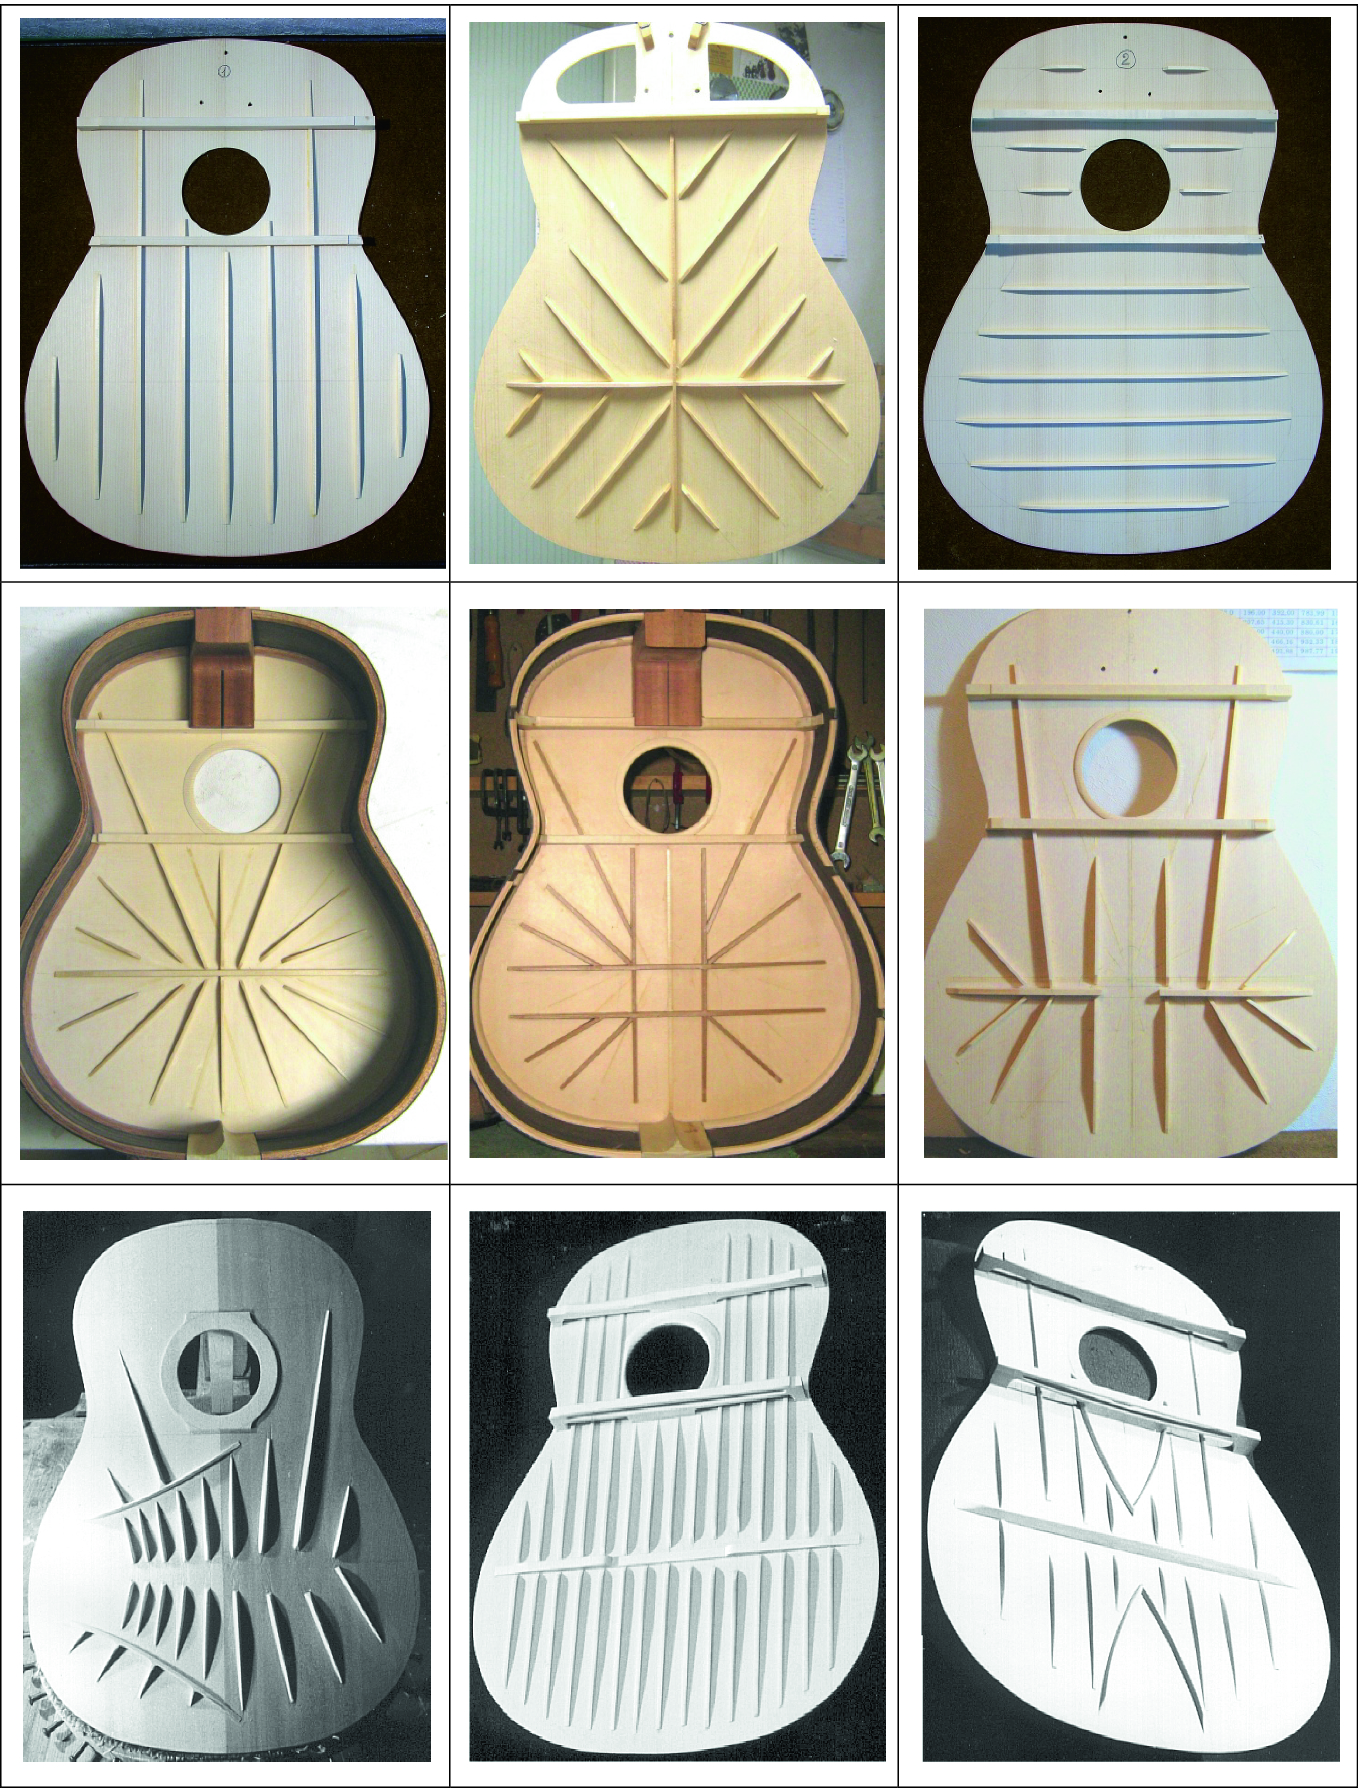
\includegraphics[width=0.4\textwidth]{img/catene.png}

\noindent
Da ciò discende che un importante apporto lo deve donare lo strumentista che in vece del compositore e tenendo a mente il suo obiettivo finale (ovvero la buona riuscita del brano e il comprendere al meglio il proprio strumento) deve studiare la metodologia più appropriata per il posizionamento e la realizzazione dello stesso. Si propone dunque di allegare al brano stesso delle caratteristiche fondamentali che il posizionamento di attuatore e sensore devo far risaltare, rendendo cosí giustizia alle composizioni che ne fanno uso. Attreverso strumenti come le figure di Chladni\footnote{tecnica che grazie alla vibrazione di una lastra permette di visualizzare i punti nodali della stessa, ovvero quei punti in cui l'ampiezza della vibrazione è virtualmente nulla} si può ad esempio effettuare la ricerca dei punti nodali dello strumento, rendendo il lavoro più semplice allo strumentista; ogni strumento avrà quindi dei suoi punti che faranno espletare al meglio risultati analoghi. Bisogna quindi precisare che la ricerca in questa direzione cercando di sfruttare lo strumento nel miglior modo possibile dovrà esser seguita dal compositore e che egli dovrà fornire strumenti adeguati per far preparare lo strumentista all'esecuzione in concerto. Questi accessori saranno un vero e proprio mezzo pratico che accompagnerà e preparerà l'interprete e lo strumento all'esecuzione.


\includegraphics[width=0.4\textwidth]{img/chladni1.png}

\noindent
Si punta quindi ad una ricerca da parte dello strumentista che possa far trasparire l'intenzione compositiva anche attraverso strumenti realizzati costruttivamente in maniere differenti, anche se come al solito la ricerca di un metodo chiaro di scrittura, è il punto fondamentale del discorso che porta allo sviluppo di una nuova metodologia di scrittura del suono e della produzione dello stesso. Allo stato attuale la mancanza di trasparenza influisce negativamente su ogni aspetto musicale avvenuto dopo l'approfondita ricerca sullo strumento, mentre ci si propone di sviluppare documentazione tale da chiarire ogni dubbio dell'esecutore ogni qualvolta esso si presterà all'eseguire la composizione. È dunque il rapporto di fiducia tra il compositore e l'interprete che lega la buona riuscita a un qualcosa di totalmente nuovo ma con forti radici nella tradizione e solo attraverso una responsabilizzazione dell'esecutore nella prima fase di conoscenza del nuovo modo di scrivere egli si potrà istruire all'essere più sensibile ed ascoltare il proprio strumento. All'interno di questa prospettiva intrisa di serietà e scrupolosità nel perseguire un obiettivo verso la gestione dell'amplificazione e del feedback, l'utilizzo di un pedale resistivo\footnote{dotato di una resistenza}  da parte dell'esecutore può far veramente responsabilizzare lo stesso. Esso si renderà presto conto della potenza e del controllo che non solo con le mani ma anche con i piedi può avere sul suono, permettendo al compositore di delegare il Live Electronics quasi interamente al musicista. Ciò permetterà di asciare di fatto invariata la figura iconica del chitarrista (da solo sul palco), che puó di fatto gestire autonomamente ed interamente la parametrica complessiva della composizione.\newline

Le nuove prospettive pongono dunque nuovi limiti e nuove possibilità, e ora potendo sfruttare l'attuatore posizionato sullo strumento è facile realizzare il passaggio concettuale che pone la riproduzione del suono attraverso lo stesso. È più complesso comprendere e capire cosa poter diffondere sul piano armonico dello strumento e conseguentemente nel sistema realizzato, cercando di sfruttare al massimo il sistema ora disponibile; nel corso di questa prima parte di ricerca si è implementato  ad esempio l'algoritmo del Karplus-Strong\footnote{Kevin Karplus, Alex Strong, \emph{Digital Synthesis of Plucked-String and Drum Timbres},Computer Music Journal, Vol. 7, No. 2, Summer 1983} che diffuso dall'attuatore ha reso ancor più veritiera la resa acustica finale dello stesso\footnote{\href{https://github.com/SMERM/BN-Tedesco/tree/master/COME-02/Lezioni_in_Compresenza/20200331/Esempi_Karplus-Strong_Attuatore_su_chitarra}{Alcuni esempi del Karplus-Strong applicato al piano armonico}}.

Il compositore è dunque chiamato a selezionare e smistare le sue idee confrontandole nel modo più scientifico possibile con quelle che lo strumento gli dona, ciò può realizzarsi  solamente attraverso un'attenta e oculata scelta dei passi da compiere lungo il percorso di ricerca e composizione, che oltre a completare, devono rendere consapevole l'interprete di ciò che egli può realizzare. Se dunque è vero che il percorso verso un nuovo modo di comporre è lungo e pieno di imprevisti, quale può mai essere il miglior modo di affrontarle se non insieme ad un interprete? Si vuole quindi sottolineare attraverso ciò l'importanza nella ricerca necessaria sullo strumento e ricordando le parole di Segovia: \begin{quote} La chitarra è lo strumento più semplice da suonare, ma il più difficile da suonare molto bene.\end{quote} Si intende quindi molto chiaramente come questo strumento abbia potuto spopolare in una miriade di contesti, portandosi dietro sempre il fascino di una donna e la possenza masculina delle sue corde più gravi, passando per le corti, gli auditorium e i concerti da migliaia di persone e pur celando dentro di sé nuove possibilità pronte ad esprimersi solamente grazie alla dedizione e alla collaborazione di compositori ed esecutori. 


\newpage

%===============================================Brani ascoltati e partiture visionate

\section{ Brani ascoltati \& partiture visionate}
•\textsc{\textsf {Agostino Di Scipio}}, \emph{Ektopos}, UT Orpheus 2000\\\newline
•\textsc{\textsf {Azio Corghi}}, \emph{Consonancias y Redobles}, Universal Edition 1973\\\newline
•\textsc{\textsf {Barbara Kolb}}, \emph{ - Looking for Claudio}, Boosey \& Hawkes 1975\\\newline
•\textsc{\textsf {Benjamin Britten}}, \emph{Nocturnal After John Dowland}, Faber Music Limited 1964\\\newline
•\textsc{\textsf {Brian Ferneyhough}}, \emph{Kurze Schatten II}, Edition Peters 1983-89\\\newline
•\textsc{\textsf {Brian Ferneyhough}}, \emph{no time(at all)}, Edition Peters 2003\\\newline
•\textsc{\textsf {Bruno Maderna}}, \emph{Y Después}, Ricordi 1971\\\newline
•\textsc{\textsf {Bruno Maderna}}, \emph{Serenata per un satellite}, Ricordi 1969\\\newline
•\textsc{\textsf {Fabio Vacchi}}, \emph{Plynn}, 1987\\\newline
•\textsc{\textsf {Fabrizio Casti}}, \emph{ L' 'Anima Visionaria}, UT Orpheus 2000\\\newline
•\textsc{\textsf {Fausto Romitelli}}, \emph{Trash TV Trance}, Ricordi 2002\\\newline
•\textsc{\textsf {Fausto Romitelli}}, \emph{Solare}, Ricordi 1984\\\newline
•\textsc{\textsf {Fausto Romitelli}}, \emph{La lune et les eaux}, Ricordi 1991\\\newline
•\textsc{\textsf {Fausto Romitelli}}, \emph{Seascape}, Ricordi 1994\\\newline
•\textsc{\textsf {Fausto Romitelli}}, \emph{Coralli}, Ricordi 1987\\\newline
•\textsc{\textsf {Fausto Romitelli}}, \emph{Highway to hell}, Ricordi 1984\\\newline
•\textsc{\textsf {Federico Bonacossa}}, \emph{Shikantaza}, Cyklos 2005\\\newline
•\textsc{\textsf {Franco Donatoni}}, \emph{Algo n.2}, Ricordi 1993\\\newline
•\textsc{\textsf {Giacinto Scelsi}}, \emph{Ko-Tha}, Salabert 1962\\\newline
•\textsc{\textsf {Helmut Lachenmann}}, \emph{Salut für Caudwell}, Edition Breitkopf 1977\\\newline
•\textsc{\textsf {Luciano Berio}}, \emph{Sequenza XI}, Universal Edition 1988\\\newline
•\textsc{\textsf {Maurizio Pisati}}, \emph{Set7}, Kairos 2017\\\newline
•\textsc{\textsf {Sylvano Bussotti}}, \emph{Ultima rara (pop song)}, Ricordi 1970\\\newline
•\textsc{\textsf {Tristan Murail}}, \emph{Tellur}, Transatlantiques 1977\\\newline
•\textsc{\textsf {Tristan Murail}}, \emph{Vampyr!}, Editions Henry Lemoine 1984\\\newline
•\textsc{\textsf {Toru Takemitsu}}, \emph{12 songs for guitar}, Schott 2005\\\newline
•\textsc{\textsf {Toru Takemitsu}}, \emph{All In Twilight}, Schott 1993\\\newline
•\textsc{\textsf {Toru Takemitsu}}, \emph{Equinox}, Schott 1993\\\newline
•\textsc{\textsf {Toru Takemitsu}}, \emph{To the edge of dream}, Schott 1983\\\newline


\vfill\null
\columnbreak

%===============================================Bibliografia & sitografia
\section{ Bibliografia \& sitografia}
•\textsc{\textsf {Arturo Tallini}}, \emph{MusicaIncerta, un'introduzione alla musica contemporanea per chitarra}, UT Orpheus 2000\\\newline
•\textsc{\textsf {Arturo Tallini}}, \emph{Ma! - Con le note scritte}, Fronimo N° 185 Gennaio 2019\\\newline
•\textsc{\textsf {Curt Sachs}}, \emph{Storia degli strumenti musicali}, Mondadori 1980\\\newline
•\textsc{\textsf {Emilio Pujol}}, \emph{El dilemmma del sonido en la guitarra}, Ricordi 1979\\\newline
•\textsc{\textsf {Carlo Carfagna, Michele Greci}}, \emph{Chitarra, storia e immagini}, Fratelli Palombi Editori 2000\\\newline
•\textsc{\textsf {Karlheinz Stockhausen}}, \emph{Sulla musica, a cura di Robin Maconie}, Marion Boyars 1989\\\newline
•\textsc{\textsf {Kevin Karplus, Alex Strong}}, \emph{Digital Synthesis of Plucked-String and Drum Timbres},Computer Music Journal, Vol. 7, No. 2,
Summer 1983\\\newline
•\textsc{\textsf {Michelangelo Lupone}}, \emph{\href{https://www.youtube.com/watch?v=btioUhxSoCM}{Poetica e tecnica del Feed-back per l’aumentazione degli strumenti}}, Biennale CIMM 2019\\\newline
•\textsc{\textsf {Rita Torres, Paulo Ferreira-Lopes}}, \emph{Towards Overcoming the Guitar's Color Research Gap}, CITAR 2014\\\newline
•\textsc{\textsf {Jonathan Godfrey}}, \emph{Principles of Idiomatic Guitar Writing},  2013\\\newline
•\textsc{\textsf {John Schneider}}, \emph{The Contemporary Guitar},  University of California Press 1985\\\newline

\vfill\null
\columnbreak
%===============================================Indice delle figure

\section{ Indice delle figure}
\hspace*{10mm}

\begin{enumerate}

\item \emph{Spaccato e parti di una chitarra classica}\newline
\item \emph{Frammento di \textit{Ektopos} di Agostino Di Scipio}\newline
\item \emph{Sensore piezo-elettrico ed attuatore installati su di una chitarra classica}\newline
\item \emph{IR della prima posizione testata del sistema sensore-attuatore}\newline
\item \emph{Frammento della legenda preparatoria agli Studi per chitarra classica}\newline
\item \emph{Classificazione dei luoghi percussivi della chitarra classica}\newline
\item \emph{Varie tipologie di \textit{catenatura} di una chitarra classica}\newline
\item \emph{Figure di Chladni di una chitarra classica a diverse frequenze}\newline

\end{enumerate}

\end{multicols*}

\textit{Il testo qui presentato è a corredo dal materiale elaborato durante il primo anno di Biennio 2019-2020 del corso di Composizione Musicale Elettroacustica del Conservatorio di Roma, Santa Cecilia, reperibile al \textbf{\href{https://github.com/SMERM/BN-Tedesco/}{seguente link}}.}

\end{document}
